\section{Measured results and decision}

% Generated by stage1/plot_controls.py; do not edit numerical values here.
% analytic-checks.json SHA-256: 052e4635061b7596c9093604ea3413d86902094092e41997acb327e9e1dba4c4
\subsection{Analytic controls and original-profile audit}
The existing test suite passes 40 tests and 34 subtests
(\path{../results/tests.log}),
including the explicit multimode convolution check with nonzero mean flow.
For plane waves $A=0.6$, $k=0,\pm3$, the largest RHS error is
$1.43\times10^{-12}$ and the largest propagated complex error at
$\xi=2$ is $1.45\times10^{-13}$.
The moving NLS control at $N=2048$, $L=80$, $\mu=2$, $s=1$ has the errors
in Table~\ref{tab:nls}. Successive observed orders approach four
(Figure~\ref{fig:controls}a). Here $p=\log(e_{\rm coarse}/e_{\rm fine})/
\log(h_{\rm coarse}/h_{\rm fine})$; these are exact-solution errors, not
estimates inferred from conservation.

\begin{table}[htbp]
\centering
\caption{Moving NLS complex relative L2 error at $\xi=2$. The ratio compares
with the preceding coarser step.}\label{tab:nls}
\begin{tabular}{rrrr}
\toprule
$\Delta\xi$ & Error & Ratio & Order $p$ \\
\midrule
0.04 & $3.79\times10^{-4}$ & --- & --- \\
0.02 & $2.56\times10^{-5}$ & 14.767 & 3.884 \\
0.01 & $1.65\times10^{-6}$ & 15.548 & 3.959 \\
0.005 & $1.04\times10^{-7}$ & 15.823 & 3.984 \\
\bottomrule
\end{tabular}
\end{table}

A recomputed moving Dysthe profile ($\epsilon=0.025$, $\mu=2$, $s=1$,
$N=4096$, $L=160$) has full residual
$2.06\times10^{-11}$.
At $\xi=2$ and $\Delta\xi=0.000625$,
its raw complex error against the declared traveling solution is
$9.66\times10^{-12}$.

On two independent multimode test fields, full-RHS directional rates of
$\mathcal A,\mathcal M,\mathcal E$ are at most $3.24\times10^{-12}$
in absolute value per unit $\xi$, while the near-cutoff Galerkin energy
rate is $5.92\times10^{-5}$. This explicitly exposes a
projection contribution to invariant drift.


All 28 original stored profiles were independently re-audited on their
original $N=2048$, $L=160$ grid (Figure~\ref{fig:controls}b).
Although every retained residual is at most $4.36\times10^{-11}$,
22 full periodic residuals exceed the current $10^{-8}$ gate.
The largest is $6.12\times10^{-3}$ at
$(\epsilon,\mu,s)=(0.15,3,0)$;
16 profiles also exceed the $\epsilon\max|F|\leq0.1$ design screen.
These results require requalification or finer profile grids; they do not
establish physical instability or nonexistence. The CSV audit retains the
per-profile hashes, residual components, and separate gate decisions.

\begin{figure}[htbp]
\centering
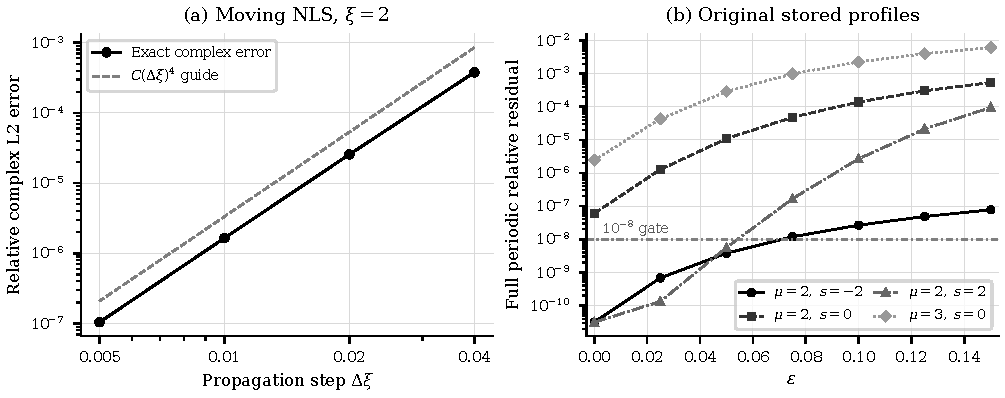
\includegraphics[width=\linewidth]{figures/controls.pdf}
\caption{Analytic propagation control and original-profile full-equation audit.
The dashed fourth-order guide is scaled for visibility. The profile gate
uses the full residual of \eqref{eq:residual}, not the iteration residual.}
\label{fig:controls}
\end{figure}


\subsection{Separate propagation-step and grid checks}

The reused October runs contain 28 trajectories, distinct from the 28 stored branch profiles. Their core and campaign hashes still match the current propagator. Ten new full-horizon trajectories and a two-trajectory short benchmark were run locally; no scheduler or paid compute was used. All new Dysthe cases use $\epsilon=.025$, $\mu=2$, $s=0$, and $0\leq\xi\leq20$. The odd perturbation is $F[1+10^{-3}(\tau/2)e^{-(\tau/2)^2}]$, projected before propagation.

The step table compares successive runs at fixed $L=160$, $N=4096$. Its numbers are maxima over integer samples of $\xi$, normalized by the fine profile norm.

\begin{center}
\small
\begin{tabular}{lrrr}
\toprule
$\Delta\xi$ pair & Control field & Odd field & Signed shape \\
\midrule
0.005 / 0.0025 & $5.96\times10^{-6}$ & $5.96\times10^{-6}$ & $2.08\times10^{-10}$ \\
0.0025 / 0.00125 & $2.96\times10^{-7}$ & $2.96\times10^{-7}$ & $7.90\times10^{-12}$ \\
0.00125 / 0.000625 & $1.66\times10^{-8}$ & $1.66\times10^{-8}$ & $4.65\times10^{-13}$ \\
\bottomrule
\end{tabular}
\end{center}


The final-control observed orders are 4.335 and 4.154. At the smallest historical pair, the maximum raw-field difference is $1.66\times10^{-8}$. Conservation cannot expose this phase-sensitive error by itself.

\begin{center}
\small
\begin{tabular}{lrr}
\toprule
Fixed-domain grid pair & Odd field & Signed shape \\
\midrule
$L=160$: $4096/8192$ & $2.45\times10^{-14}$ & $1.51\times10^{-14}$ \\
$L=320$: $8192/16384$ & $2.67\times10^{-13}$ & $2.31\times10^{-14}$ \\
\bottomrule
\end{tabular}
\end{center}


Both grid comparisons fix $\Delta\xi=.000625$; Fourier interpolation puts each pair on the finer grid. Thus enlarging the domain is not being confused with raising the retained physical wavenumber cutoff.

\begin{figure}[htbp]\centering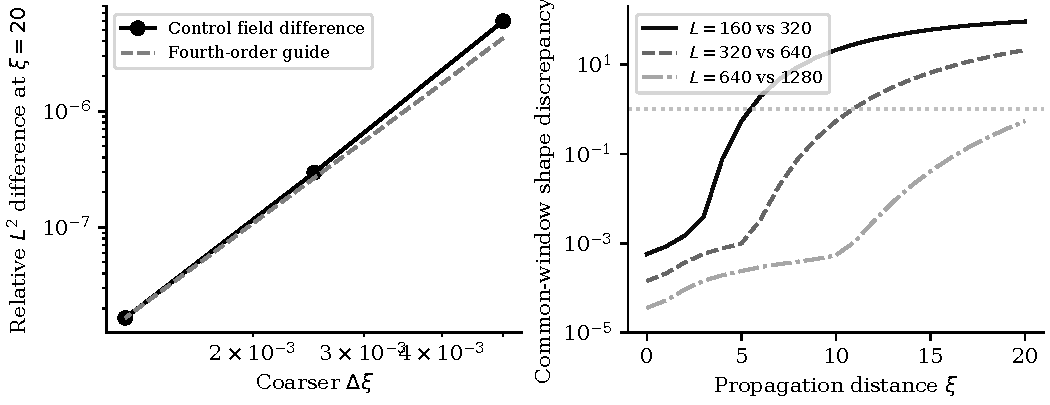
\includegraphics[width=\linewidth]{figures/convergence.pdf}\caption{Step convergence and signed weak-response domain discrepancies. The domain panel uses the fine response norm on the common window; the dotted line is a one-percent comparison target, not a rigorous bound.}\end{figure}

\subsection{Domain sensitivity and the weak odd response}

The domain sequence doubles $L=160,320,640,1280$ at fixed $L/N=160/4096$ and $\Delta\xi=.000625$. Each periodic profile is recomputed. The table gives results at $\xi=20$; shape and core differences are normalized by the fine carrier profile on the common window, and the last column divides by the weak shape on that window. The core is $|\tau|<20$.

\begin{center}
\small
\begin{tabular}{lrrrr}
\toprule
$L$ pair & Initial profile & Signed shape & Core & Shape ratio \\
\midrule
160 / 320 & $1.54\times10^{-6}$ & $2.19\times10^{-5}$ & $8.76\times10^{-6}$ & 91\% \\
320 / 640 & $3.85\times10^{-7}$ & $6.69\times10^{-6}$ & $2.60\times10^{-7}$ & 21\% \\
640 / 1280 & $9.63\times10^{-8}$ & $1.75\times10^{-7}$ & $1.64\times10^{-10}$ & 0.538\% \\
\bottomrule
\end{tabular}
\end{center}


The previously quoted $67.4\%$ discrepancy for $160/320$ used the entire fine-domain response as denominator. The common-window denominator in this table gives $91.1\%$. These are the same field discrepancy with different denominators, not conflicting results. For $320/640$ the full-domain denominator gives $20.6\%$, compared with $21.0\%$ on the common window.

The $320/640$ response outside the smaller period has normalized norm $6.69\times10^{-6}$, nearly equal to the discrepancy. Periodizing that exterior reduces the discrepancy to $1.95\times10^{-7}$. Together with the response spectrum and travel times, this strongly supports radiation wrapping as the principal mechanism. Periodic nonlocal profile differences and later nonlinear interactions remain present; folding is only a diagnostic.

At $L=1280$, the final raw perturbation/control distance is $2.36\times10^{-4}$, while the shape distance after fitting is $3.25\times10^{-5}$. The fitted translation is $2.74\times10^{-4}$ and constant phase $6.77\times10^{-5}$ radians. Translation and phase therefore account for most of the raw response, while the remaining signed deformation still includes radiation.

\begin{figure}[htbp]\centering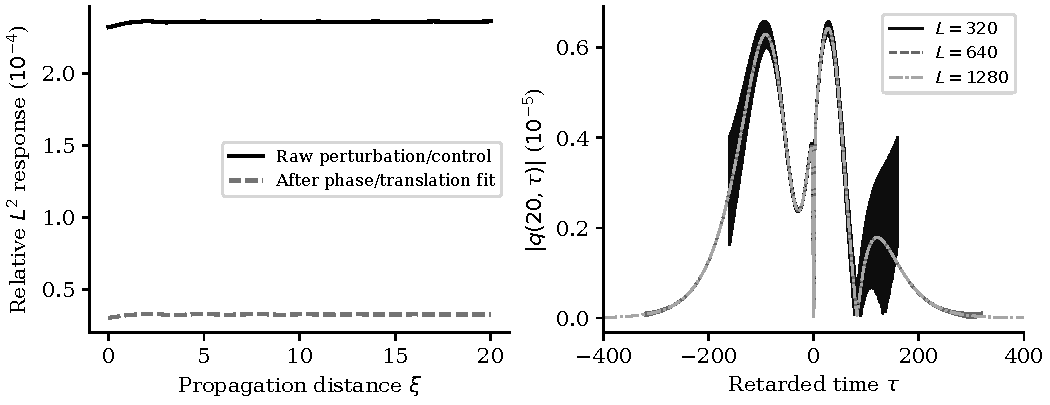
\includegraphics[width=\linewidth]{figures/shape-and-drift.pdf}\caption{Raw versus fitted response and the final signed-response magnitude. Nearly equal scalar shape norms can hide substantially different radiation fields; the convergence tests compare the complex fields themselves.}\end{figure}

\subsection{Residuals, invariants, and resources}

The largest initial/final discarded-RHS ratio in the accepted-spacing, small-step cases is $9.29\times10^{-12}$. This is an instantaneous resolution diagnostic, not a time-integrated error bound. The following invariant maxima cover both control and odd trajectories; energy and momentum are the continuum functionals rather than assumed exact discrete invariants.

\begin{center}
\small
\begin{tabular}{lrrr}
\toprule
$L$ & Action drift & Energy drift & Momentum drift \\
\midrule
160 & $8.66\times10^{-13}$ & $2.72\times10^{-12}$ & $6.74\times10^{-11}$ \\
640 & $6.29\times10^{-13}$ & $1.98\times10^{-12}$ & $6.74\times10^{-11}$ \\
1280 & $7.30\times10^{-13}$ & $2.30\times10^{-12}$ & $6.73\times10^{-11}$ \\
\bottomrule
\end{tabular}
\end{center}


The five new full-horizon cases used 809.2 process-wall seconds in total, with peak recorded process RSS 177.9 MiB. Some cases ran concurrently, so these durations are not elapsed session time. The benchmark used less than one second. Every saved field was finite. The existing large-window sech initial guess emitted one benign cosh-overflow warning in its vanishing tails; it did not produce nonfinite profiles or trajectories.

\subsection{Recommendation and accuracy limits}

\textbf{Go for the next small initial-data simulator, after review, using this periodic equation and per-case qualification.} The reference passes analytic controls, independent residual checks, fourth-order step convergence, and independent grid convergence. No change to the equation or propagator was needed. The added diagnostics separate symmetry drift and identify the domain failure mechanism.

For an illustrative one-percent signed weak-response agreement target, the sampled horizons of the smaller windows are $\xi\leq 5$ for $L=160$, $\xi\leq 10$ for $L=320$, and $\xi\leq 20$ for $L=640$, each assessed against the next doubled domain. These are measured sample-wise agreements for this perturbation, not rigorous error bars or universal domain choices.

The final $640/1280$ common-window shape discrepancy is $1.75\times10^{-7}$, or 0.538\% of this weak shape response. A full-domain initial-data simulator must preserve phase, translation, and radiation and expose numerical-resolution checks. New focusing, modulation, and bandwidth ranges need their own convergence evidence.

\textbf{No-go for a large training corpus or FNO training now.} The original $L=160$, $\xi=20$ setup is not qualified as an isolated weak-radiation reference. The entire legacy profile library is not qualified either. The next stage should implement a small plug-and-play simulator with a finite, explicitly tested input range; dataset generation and learning require a later decision. Short persistence does not establish soliton discovery or stability.
